\documentclass[../p111main.tex]{subfiles}
\graphicspath{{\subfix{../figures/}}}

\begin{document}

\chapter{Two-Body Dynamics}
\section{Two-Body Dynamics}
Now that we've developed the Lagrangian formalism in reasonable depth, we'll take a look at what we can actually do with it.
Broadly speaking, interactions between a pair of objects fall into two different categories: bound states and scattering states.
In a bound state the objects ``meet'' infinitely times and stay relatively close together, while in a scattering state objects meet once and never again.

Either way, the two-body problem has the Lagrangian
\[ L = \frac{1}{2} (m_1 + m_2) |\dot{\mbf{R}}|^2 + \frac{1}{2} \frac{m_1m_2}{m_1 + m_2} |\dot{\mbf{r}}|^2 - U(r), \]
where $\mbf{R}$ is the center of mass position and $\mbf{r}$ is the displacement from $\mbf{r}_1$ to $\mbf{r}_2$.
We can see that the COM momentum is conserved, so we can safely look at the COM frame to get
\begin{align*}
    L &= \frac{1}{2} \frac{m_1 m_2}{m_1 + m_2} |\dot{\mbf{r}}|^2 - U(r) \\
    &= \frac{1}{2} \mu \left( \dot r^2 + r^2 \dot \theta^2 + r^2 \sin^2 \theta \,\dot \phi^2 \right) - U(r).
\end{align*}
So the two-body system is equivalent to a single-particle system with reduced mass $\mu$ and potential $U(r)$.
We can further simplify this Lagrangian by recognizing that all of the interactions between the two bodies are in the same plane, meaning we can restrict our reference frame to $\theta = \pi / 2$ and $\dot \theta = 0$ with no problems.
So now we have
\[ L = \frac{1}{2} \mu \left( \dot r^2 + r^2 \dot \phi^2 \right) - U(r). \]
Finally, we can note that $\phi$ is cyclic and define the conserved $p_\phi = \ell = \mu r^2 \dot \phi$ to write the Lagrangian purely in terms of $r$ and $\dot r$.
This gives us the kind of spherical symmetry we'd expect from a central potential!

More interesting to us for now, though, is the Hamiltonian (which is also conserved):
\[ H = T + U = \frac{1}{2} \mu \dot r^2 + \frac{\ell^2}{2\mu r^2} + U(r). \]
Since the latter two terms depend only on $r$ we'll bring them together into one ``effective potential'' $U_\textrm{eff}(r)$, turning this into
\[ H = \frac{1}{2} \mu \dot r^2 + U_\textrm{eff}(r). \]
When plotted, $U_\textrm{eff}(r)$ looks like the well-known attraction potential curve---asymptotes at $r=0$ and $U_\text{eff}(r) = 0$ with a little dip below the horizontal axis.
Oscillations about the bottom of the ``well'' with $U_\textrm{eff}(r) < 0$ correspond to elliptical trajectories, while ones with $U_\textrm{eff}(r) > 0$ are hyperbolic.
The first term in $U_\textrm{eff}(r)$ serves as a ``centrifugal barrier''---if the masses get too close, conservation of angular momentum slingshots them away from one another.

With constant $H$ we can interpret the above equation as a separable differential equation with solution
\[ t(r) - t(r_0) = \pm \sqrt{\frac{\mu}{2}} \int_{r_0}^{r} \frac{dr'}{\sqrt{H - U_\textrm{eff}(r')}}. \]
The $\pm$ here accounts for the two possible orientations of the orbit.
But $t(r)$ isn't quite what we want---employing a change of variables $dt = (\mu r^2 / \ell) d\phi$ gives
\[ \phi(r) - \phi(r_0) = \pm \frac{\ell}{\sqrt{2\mu}} \int_{r_0}^{r} \frac{dr'}{r'^2} \frac{1}{\sqrt{H - U_\textrm{eff}(r')}}. \]
This equation will be central to our study of two-body dynamics.

\section{Kepler Orbits}
Now we'll look at the case of $U(r) = -\alpha / r$, which might correspond to a gravitational or electrostatic potential.
Let $r_0$ denote the minimum of $U_\textrm{eff}(r)$, so in this case we'd find that $r_0 = \ell^2 / \mu \alpha$.
The integral from the previous section turns out to be
\[ \phi(r) - \phi(r_0) = \pm \arcsin \left( \frac{\alpha r - \ell^2 / \mu}{r \sqrt{\alpha^2 + 2E \ell^2 / \mu}} \right). \]
By convention we define $(r_0) = \pi / 2$.
It follows that
\[ \cos \phi = \pm \frac{\alpha r - \ell^2 / \mu}{r \sqrt{\alpha^2 + 2 E \ell^2 / \mu}}, \]
and solving for $r$ gives
\[ r(\phi) = \frac{\ell^2}{\mu \alpha} \frac{1}{1 \mp \varepsilon \cos \phi}, \qquad \varepsilon \equiv \sqrt{1 + \frac{2E\ell^2}{\mu \alpha^2}}, \]
where by convention we take $\mp = +$ so that $r(0) = r_\textrm{min}$.
The quantity $\varepsilon$ is called the eccentricity, and it denotes the path's deviation from circularity (which is at $\varepsilon = 0$).
Bound orbits have $\varepsilon < 1$.

Notice that if we substitute $r = \sqrt{x^2 + y^2}$ and $\cos \phi = x / r$ we get
\[ \frac{(x+d)^2}{a^2} + \frac{y^2}{b^2} = 1, \qquad a = \frac{l^2 / \mu \alpha}{1 - \varepsilon^2}, \quad b = a \sqrt{1 - \varepsilon^2}, \quad d = a\varepsilon. \]
This proves Kepler's first law, that gravitational orbits are elliptical.
The three parameters are the semimajor axis, the semiminor axis, and the center-focus distance, respectively.

Kepler's second law states that orbits sweep out equal areas in equal times---approximating each $dA$ as a triangle gives
\[ dA = \frac{1}{2} r \, (r d\phi) \;\implies\; \frac{dA}{dt} = \frac{1}{2} r^2 \dot \phi^2 = \frac{\ell}{2\mu}. \]
As for Kepler's third law we have
\[ (\textrm{period})^2 = \left( \frac{\textrm{area}}{dA / dt} \right)^2 = \frac{4\pi^2 a^3}{\ell^2} \cdot \mu^2 a(1 - \varepsilon^2) = \frac{4\pi^2 a^3}{\ell^2} \frac{\ell^2}{\mu \alpha}, \]
meaning $(\textrm{period})^2 \propto a^3$.

Finally, let's bring this back to our original two-body problem in the center-of-mass frame.
Here we have
\[ \mbf{R}_\textrm{CM} = \frac{m_1 \mbf{r}_1 + m_2 \mbf{r}_2}{m_1 + m_2} = 0; \]
together with $\mbf{r} = \mbf{r}_1 - \mbf{r}_2$ we get a system of equations whose solution is
\[ \mbf{r}_1 = \frac{m_2}{m_1 + m_2} \mbf{r}, \qquad \mbf{r}_2 = -\frac{m_1}{m_1 + m_2} \mbf{r}. \]
So both bodies have the same orbital shape (ellipses with the same orientation and eccentricity), but are opposite in position along those orbits.

As a side note, it turns out (by Bertrand's theorem) that all this theory of closed orbits is only possible for central potentials that look like
\[ U(r) = -\frac{\alpha}{r}, \quad U(r) = kr^2. \]
Small deviations from these potentials give \textit{approximately} elliptical orbits.
The actual behavior of such a system is quite complex!
(Think about phenomena like orbital precession.)

\section{Particle Scattering}
Now we'll move into a discussion about scattering states.
First we will show that, very conveniently, all trajectories in a central potential are symmetric about a line between the origin and the point of closest approach.
Let $B$ denote this point and let $A$ and $C$ be points on opposite sides of $B$ satisfying $r_A = r_C$.
We'll show that the $\Delta \phi$ from $B$ satisfy $\Delta \phi_{BA} = \Delta \phi(CB)$:
\[ \Delta \phi_{BA} = -\frac{\ell}{\sqrt{2\mu}} \int_{r_A}^{r_B} \frac{dr'}{r'^2} \frac{1}{\sqrt{E - U_\textrm{eff}(r')}} = -\frac{\ell}{\sqrt{2\mu}} \int_{r_A}^{r_C} (\cdots) = \frac{\ell}{\sqrt{2\mu}} \int_{r_C}^{r_A} (\cdots) = \Delta \phi_{CB}. \]
Combined with the fact that both branches of the trajectory have the same shape, we conclude that the trajectory is symmetric.

Another important fact is that scattering in a central potential is elastic, so kinetic energy is conserved in the infinite ``before'' and ``after'' of the collision.
This has to do with the fact that $U_\textrm{eff}(\infty)$ must be finite to allow for unbound trajectories; we'll take $U_\textrm{eff}(\infty) = 0$ for the remainder of our discussion.

Each scattering trajectory is determined entirely by the energy $E$ and angular momentum $\ell$ relative to the center of the potential.
We could also choose other pairs of constants, like the initial speed $v_\infty$ and the impact parameter $b$, the particle's center-offset as it approaches from infinity.
(These two pairs of parameters are related by $E = \mu v_\infty^2 / 2$ and $\ell = \mu v_\infty b$.)
The potential then determines the scattering angle $\theta$ as a function of these constants.

There's a couple of choices of $U(r)$ that are particularly relevant to us.
The first is the case of hard sphere scattering, for which $U(r)$ is infinite within a radius $a$ and zero outside.
If $b > R$ then the problem is easy---the incident particle never ``hits'' the potential and $\theta = 0$.
Otherwise, if $\alpha$ is the angle the initial trajectory makes with the line of symmetry, then we have $\sin \alpha = b / R$ and
\[ \sin \left( \frac{\pi}{2} - \frac{\theta}{2} \right) = \frac{b}{R} \;\implies\; \theta = 2 \arccos \left( \frac{b}{R} \right). \]
So for a hard sphere the scattering angle is
\[ \theta = \begin{cases} 2 \arccos (b / R) & b \leq R, \\ 0 & b > R. \end{cases} \]
\parbox{0.6\textwidth}{
    Now let's look at Rutherford scattering, for which $U(r) = -\alpha / r$.
    We know, from previous discussion, that our particle will follow a hyperbolic trajectory; such a trajectory is drawn at right.
    We know
    \[ r(\phi) = \frac{\ell^2}{\mu \alpha} \frac{1}{1 + \varepsilon \cos \phi}, \quad \varepsilon \geq 1, \]
    and if $r \to \infty$ we get $\cos(\pi - \phi_0) = -1 / \varepsilon$ and $\cos \phi_0 = 1 / \varepsilon$.
    We can relate this to our parameters using
    \[ \varepsilon = \sqrt{1 + \frac{2E \ell^2}{\mu \alpha^2}} = \sqrt{1 + \frac{\mu^2 b^2 v_\infty^4}{\alpha^2}}. \]
    Also, because $1 / \varepsilon = \cos \phi_0 = \cos \left( \pi / 2 - \theta / 2 \right) = \sin(\theta / 2)$,
}\parbox{0.4\textwidth}{
    \quad\;
    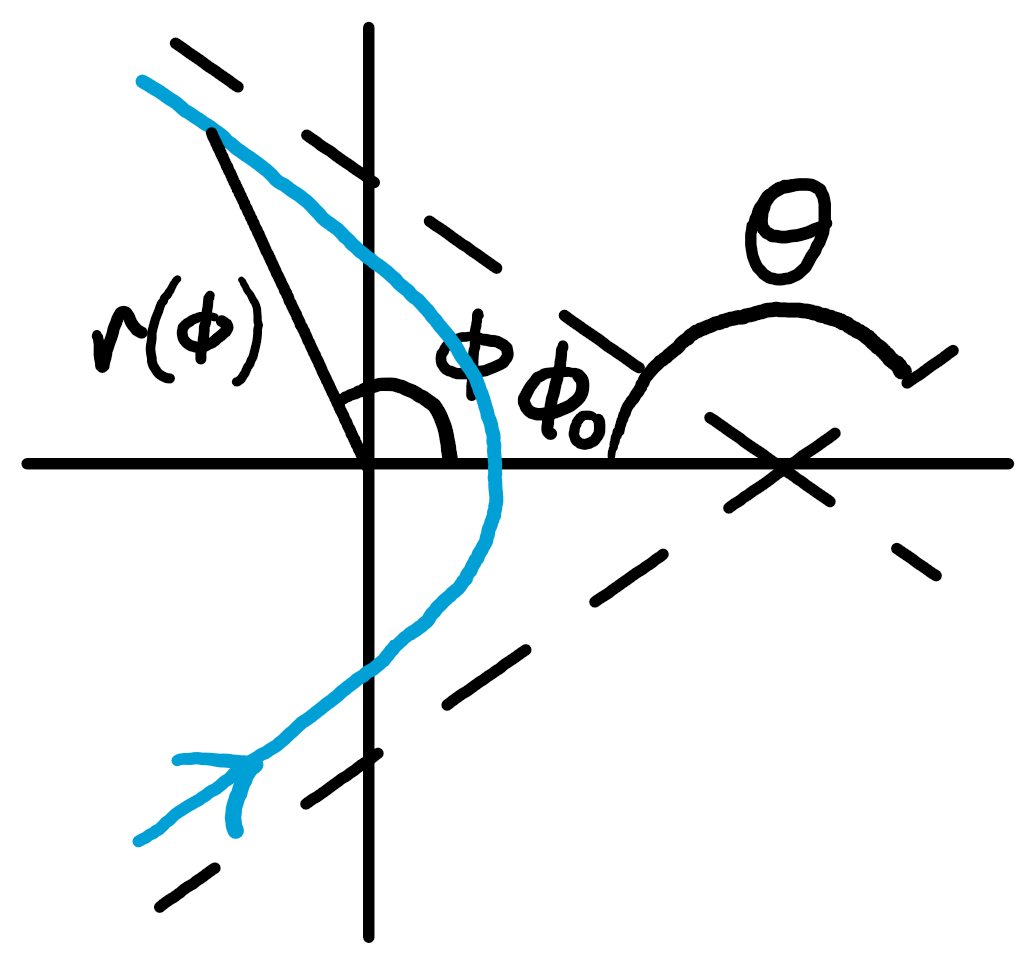
\includegraphics[width=0.35\textwidth]{rutherfordScattering.png}
}

\[ \frac{1}{\sin^2 (\theta / 2)} = 1 + \cot^2 \frac{\theta}{2} = \varepsilon^2 = 1 + \frac{\mu^2 b^2 v_\infty^2}{\alpha^2}. \]
So we end up with the scattering angle
\[ \theta = 2 \arctan \left( \frac{|\alpha|}{\mu b v_\infty^2} \right); \]
we would've gotten the same result with a repulsive potential rather than an attractive one.

\section{Beam Scattering}
All this theory is great, but it has some practical limitations.
In particular, we'd normally employ lots of different particles in any given scattering experiment we'd do, and we can't aim them precisely.
So we don't exactly know $b$, $v_\infty$, and $\theta$ for each particle!

To characterize the behavior of a beam of particles, we define the current $I$ and current density $\mbf{J}$ so that
\[ dI = \mbf{J} \cdot \hat n \,d\sigma = J \,d\sigma, \]
where $d\sigma$ is an infinitesimal cross section of the beam.
The number of particles incident on an infinitesimal target in a time $dt$ is $N_\textrm{inc} = J \,d\sigma dt$; each $d\sigma$ scatters at a range of angles $[0, \, \theta + d\theta]$.

Suppose we have a detector with area $dA = r^2 d\Omega$ that's just big enough to catch all of these scattered particles when orthogonal to the beam.
Here $r$ is the distance from the detector to the potential's center at $r=0$, and $d\Omega = \sin \theta \,d\theta d\phi$ is the solid angle subtended by the detector when viewed from $r=0$.
There are $N_\textrm{det} = J_\textrm{det} \,dA dt$ particles detected in a time $dt$, and since $N_\textrm{inc} = N_\textrm{det}$ we have
\begin{align*}
    J_\textrm{det} dA &= J_\textrm{inc} d\sigma \\
    J_\textrm{det} r^2 d\Omega &= J_\textrm{inc} d\sigma \\
    r^2 J_\textrm{det} &= J_\textrm{inc} \cdot \frac{d\sigma}{d\Omega}
\end{align*}
Thus illustrates how the scattered current $J_\text{det}$ gets thinner with distance, as the particles all scatter at slightly different angles.
The $d\sigma / d\Omega$ is called the differential cross section and has units of area---it is a measure of how many particles passing through $d\sigma$ get scattered into $d\Omega$.
A larger $d\sigma / d\Omega$ to more scattering!

To compute the differential cross section, suppose a beam is incident upon a potential with a given $b(\theta)$, and consider a width-$db$ ring of particles with impact parameter $b$.
We have $d\sigma = 2\pi b \,db$ and $d\Omega = 2\pi \sin \theta \,d\theta$, meaning
\[ \frac{d\sigma}{d\Omega} = \frac{2\pi b \,db}{2\pi \sin \theta \,d\theta} = \frac{b}{\sin\theta} \left| \frac{db}{d\theta} \right|. \]
Let us now define the total cross section
\begin{align*}
    \sigma &= \int \left| \frac{d\sigma}{d\Omega} \right| d\Omega \\
    &= 2\pi \int_0^\pi \sin\theta \frac{b}{\sin\theta} \left| \frac{db}{d\theta} \right| d\theta \\
    &= 2\pi \int_{b_\textrm{min}}^{b_\textrm{max}} b \,db \\
    &= \pi \left( b_\textrm{max}^2 - b_\textrm{min}^2 \right).
\end{align*}
For a hard sphere we get $d\sigma / d\Omega = R^2 / 4$ and $ = \pi R^2$.
(This illustrates that $\sigma$ is the ``effective area'' of the beam that gets scattered at all!)
In the case of Rutherford scattering,
\[ b(\theta) = \frac{|\alpha|}{\mu v_\infty^2} \cot \frac{\theta}{2} \]
and $\sigma = \infty$ because, strictly speaking, the range of the Coulomb potential is infinite.
A more physically interesting quantity is the differential cross section, which turns out to be
\[ \frac{d\sigma}{d\Omega} = \frac{\alpha^2}{4\mu^2 v_\infty^{4}} \frac{1}{\sin^{4} (\theta / 2)}. \]

\pagebreak

\section{Visualizing Dynamics}
Now we'll take a step back and describe some graphical methods for studying more general dynamical systems.
Starting with just one degree of freedom, the state of whatever system we're interested in can be described entirely by the behavior of $q$ and $\dot q$.
A parametric plot $(q(t), \dot q(t))$ of these two quantities is called the system's phase space.
In the case of a simple harmonic oscillator, for example, we have the conserved Hamiltonian
\[ H = \frac{1}{2} M \dot \delta^2 + \frac{1}{2} K \delta^2, \]
which takes the form of an ellipse centered at the origin.
(We call the origin here an attractor since the system seems to be oscillating around it.)
Note that conservation of the Hamiltonian ensures that there is a one-to-one mapping between $H$ and system trajectories, so given a general time-independent potential $U(x)$ we can think carefully about how the relationship between $E$ and $U(x)$ can provide us information about the system's evolution over time.

It can also be interesting to study how the behavior of a system changes as we vary its parameters.
Consider a mass-$m$ bead on a radius-$R$ hoop spinning with angular speed $\omega$.
We could show that the equilibrium points of this system are at
\[ \theta_\textrm{eq} = 0, \pi, \qquad \cos \theta_\textrm{eq} = \left( \frac{g}{R\omega^2} \right) \equiv \gamma. \]
Our analysis of this system is split into two cases.
\begin{itemize}[topsep=0pt]
    \item If $\gamma < 1$ then we only have two equilibrium points.
    The one at the bottom of the hoop is stable, while the one at the top is unstable.

    \item If $\gamma > 1$ then we have four equilibrium points.
    The ones at the top and bottom of the hoop are unstable, and the two on the sides are stable.
\end{itemize}
So as we vary our system's parameters we may create equilibrium points, destroy them, or change their stability.
We call such changes bifurcations.

Now let's take a step up and consider a system with $N$ degrees of freedom with state vector
\[ \mbf{x} = (q_1, \ldots, q_N, \,\dot q_1, \ldots, q_N). \]
Taking $n = 2N$ for the remainder of our discussion, the state space of this system is $n$-dimensional---we get two dimensions for each degree of freedom.

In general this state space is very difficult to conceptualize, even with as few as two degrees of freedom.
To visualize things we'll often take an $(n-1)$-dimensional hyperplane $S$ of this space, called a surface of section, and plot all of the points $\mbf{x}_n$ at which $\mbf{x}$ intercepts $S$.
These points are related by a Poincaré map $P$ via
\[ \mbf{x}_{k+1} P(\mbf{x}_k). \]
If $P(\mbf{x}_\star) = \mbf{x}_\star$ then $\mbf{x}_\star$ is called a fixed point of $P$; the existence of such a point indicates the existence of a closed, periodic trajectory in state space.

Even better, each conserved quantity in our system removes a dimension from state space.
For example, the state of a pair of uncoupled pendulums is described entirely by $\mbf{x} = (\theta_1, \theta_2, \dot \theta_1, \dot \theta_2)$, but because we can write $\dot \theta_2$ in terms of $H$ we can equivalently write $\mbf{x} = (\theta_1, \theta_2, \dot \theta_1, H)$.
To capture the periodicity of $\theta_1, \theta_2$ in this system we can picture our state space as a tours---$\theta_1$ might circle around the main tube of the torus, while $\theta_2$ circles about its central axis.
$\dot \theta_1$ is on the minor radius of the torus.

Consider a surface of section $S$ at $\theta_2 = 0$.
If the ratio between the frequencies of the pendulums is rational we'll see some regular behavior---only a finite number of points will ever appear on $S$.
But for irrational frequency ratios the points become dense on a circle with radius $\dot \theta_1$ (and the trajectories will ``fill in'' in the torus).
This irrational behavior is an example of quasiperiodic motion---the motion is periodic in both $\theta_1$ and $\theta_2$, but not in both.

Note that we call a system like this one separable, since we can look at the behavior of $\theta_1, \dot \theta_1$ and $\theta_2, \dot \theta_2$ (or $\theta_1, H_1$ and $\theta_2, H_2$) completely separate from one another with no problems.

\end{document}